\chapter{Phát triển ứng dụng}\label{ch:app}

\section{Tổng quan ứng dụng}
Ứng dụng được phát triển trong đề tài là một ứng dụng web tương tác (Streamlit) cho phân tích nguy cơ bệnh tim mạch, gồm dashboard, công cụ truy vấn OLAP và hệ hỗ trợ quyết định. Ứng dụng giúp người ra quyết định theo dõi tình hình bệnh tim mạch và các yếu tố nguy cơ, tìm nguyên nhân chênh lệch giữa các nhóm dân số, mô phỏng can thiệp và chọn nhóm ưu tiên khi ngân sách hữu hạn.

Thay vì đọc trực tiếp các file XPT/CSV thô, ứng dụng kết nối tới cơ sở dữ liệu MySQL qua phiên chỉ đọc và dùng bảng phân tích cuối \code{olap_exam} (cùng \code{v_nutrition} cho dữ liệu dinh dưỡng). Bảng này cung cấp dữ liệu đã làm sạch và có cấu trúc, gồm nhân khẩu học, chỉ số cơ thể, huyết áp, xét nghiệm, hồ sơ bệnh tim mạch và các thuộc tính dimension. Quy trình ETL và cấu trúc kho dữ liệu đã được trình bày ở Chương~3 và~4; chương này tập trung vào ứng dụng và các chức năng phân tích.

Ứng dụng gồm năm trang chính:
\begin{itemize}
\item Tổng quan
\item OLAP Explorer
\item Phân tích yếu tố nguy cơ
\item Hệ hỗ trợ quyết định (DSS)
\item Kho dữ liệu \& ETL
\end{itemize}
Các trang cùng hỗ trợ một quy trình ra quyết định: từ theo dõi mức tổng quan, truy vấn đa chiều, tìm nguyên nhân, đến mô phỏng và chọn phương án, cuối cùng là kiểm tra nguồn gốc dữ liệu.

\section{Các KPI chính}
Các KPI được chọn là những chỉ số tính được trực tiếp và đáng tin từ dữ liệu sẵn có, tập trung vào tỷ lệ hiện mắc bệnh tim mạch và các yếu tố nguy cơ chính.
\begin{table}[H]
\renewcommand{\arraystretch}{1.35}\setlength{\extrarowheight}{3pt}
\centering
\caption{KPI chính và định nghĩa}
\small
\begin{tabularx}{\textwidth}{|p{3.5cm}|X|r|}
\hline
\textbf{KPI} & \textbf{Định nghĩa} & \textbf{Giá trị} \\ \hline
Số người & Số bản ghi khám trong kho & 38.612 \\ \hline
Tỷ lệ mắc CVD & Có $\geq$ 1 trong: suy tim, mạch vành, đau thắt ngực, nhồi máu, đột quỵ (tự khai báo) & 11,7\% \\ \hline
Tăng huyết áp & SBP $\geq$ 130 hoặc DBP $\geq$ 80 mmHg (ACC/AHA 2017) & 42,6\% \\ \hline
Béo phì & BMI $\geq$ 30 & 40,2\% \\ \hline
SBP trung bình & Trung bình huyết áp tâm thu & 124 mmHg \\ \hline
\end{tabularx}
\end{table}
Ngoài ra, OLAP Explorer còn cung cấp: tỷ lệ cholesterol cao, tỷ lệ HDL thấp, số ca CVD, BMI, vòng eo, cholesterol, HDL và CRP trung bình. Các chỉ số như tỷ lệ tử vong, biến cố mới, chi phí điều trị hay mức tuân thủ dùng thuốc \emph{không} được đưa vào vì dữ liệu hiện có không chứa các trường cần thiết để tính một cách đáng tin cậy.

\section{Trang 1: Tổng quan}
Trang Tổng quan cung cấp bức tranh tổng hợp về sức khỏe tim mạch của quần thể khảo sát. Trang chủ yếu dành cho lãnh đạo và người quản lý cần cái nhìn nhanh (câu hỏi Q1--Q2).
\begin{figure}[H]
\centering
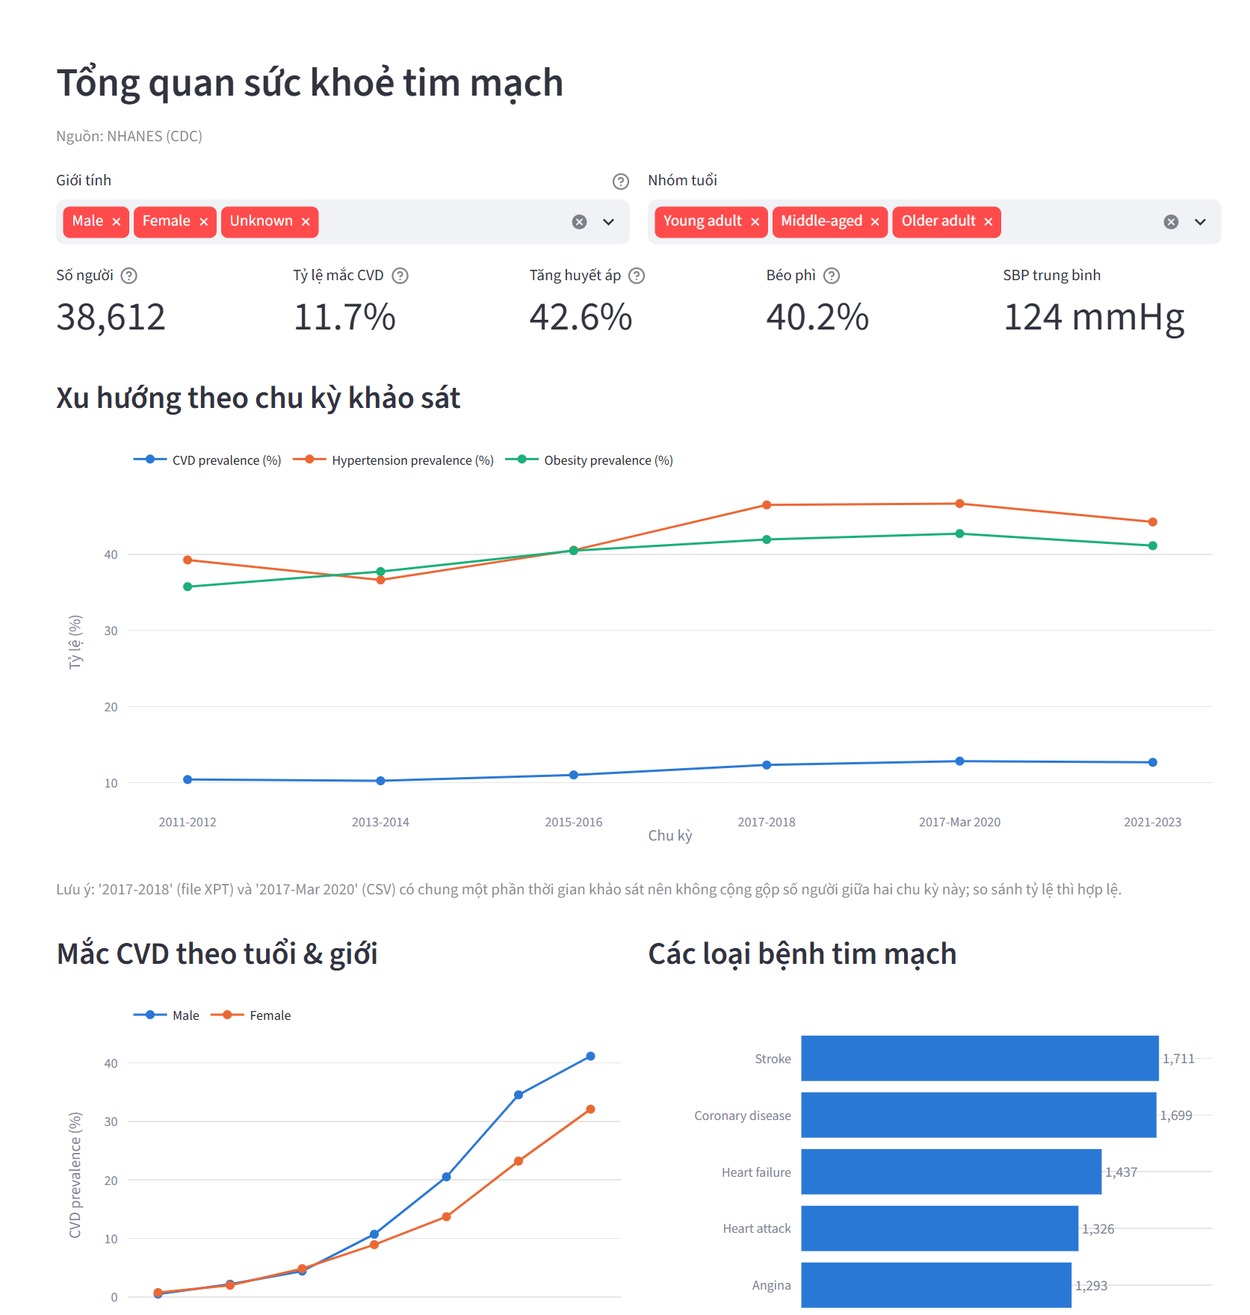
\includegraphics[width=0.7\textwidth]{figures/c_overview.png}
\caption{Trang Tổng quan}\label{fig:overview}
\end{figure}
Trang gồm năm thẻ KPI:
\begin{itemize}
\item Số người
\item Tỷ lệ mắc CVD
\item Tăng huyết áp
\item Béo phì
\item SBP trung bình
\end{itemize}
Ngoài ra trang có các biểu đồ:
\begin{itemize}
\item Xu hướng ba chỉ số (CVD, tăng huyết áp, béo phì) qua sáu chu kỳ khảo sát
\item Tỷ lệ CVD theo nhóm tuổi và giới tính
\item Số người theo từng loại bệnh tim mạch
\item Tỷ lệ CVD theo chủng tộc và theo mức thu nhập
\end{itemize}
Các biểu đồ cho phép nhanh chóng nhận ra xu hướng theo thời gian và các nhóm có tỷ lệ cao. Một số phát hiện chính: tỷ lệ CVD tăng khoảng 57 lần từ nhóm 20--29 tuổi (0,64\%) lên nhóm 80+ (36,35\%); nam cao hơn nữ (12,66\% so với 9,38\%); CVD tăng từ 10,4\% (2011--2012) lên 12,3\% (2017--2018), tăng huyết áp từ 39,3\% lên 46,5\%, béo phì từ 35,7\% lên 41,9\%; nhóm thu nhập cao nhất có tỷ lệ thấp nhất (7,00\%), nhóm thu nhập thấp có tỷ lệ cao nhất (14,12\%), tuy chưa hiệu chỉnh theo tuổi. Bộ lọc giới tính và nhóm tuổi áp dụng cho cả trang.

\section{Trang 2: OLAP Explorer}
Trang OLAP Explorer dành cho nhà phân tích muốn truy vấn đa chiều tự do mà không phải viết lại mã xử lý (câu hỏi Q2, Q9). Người dùng chọn chiều, thước đo và cách tổng hợp trên mô hình sao.
\begin{figure}[H]
\centering
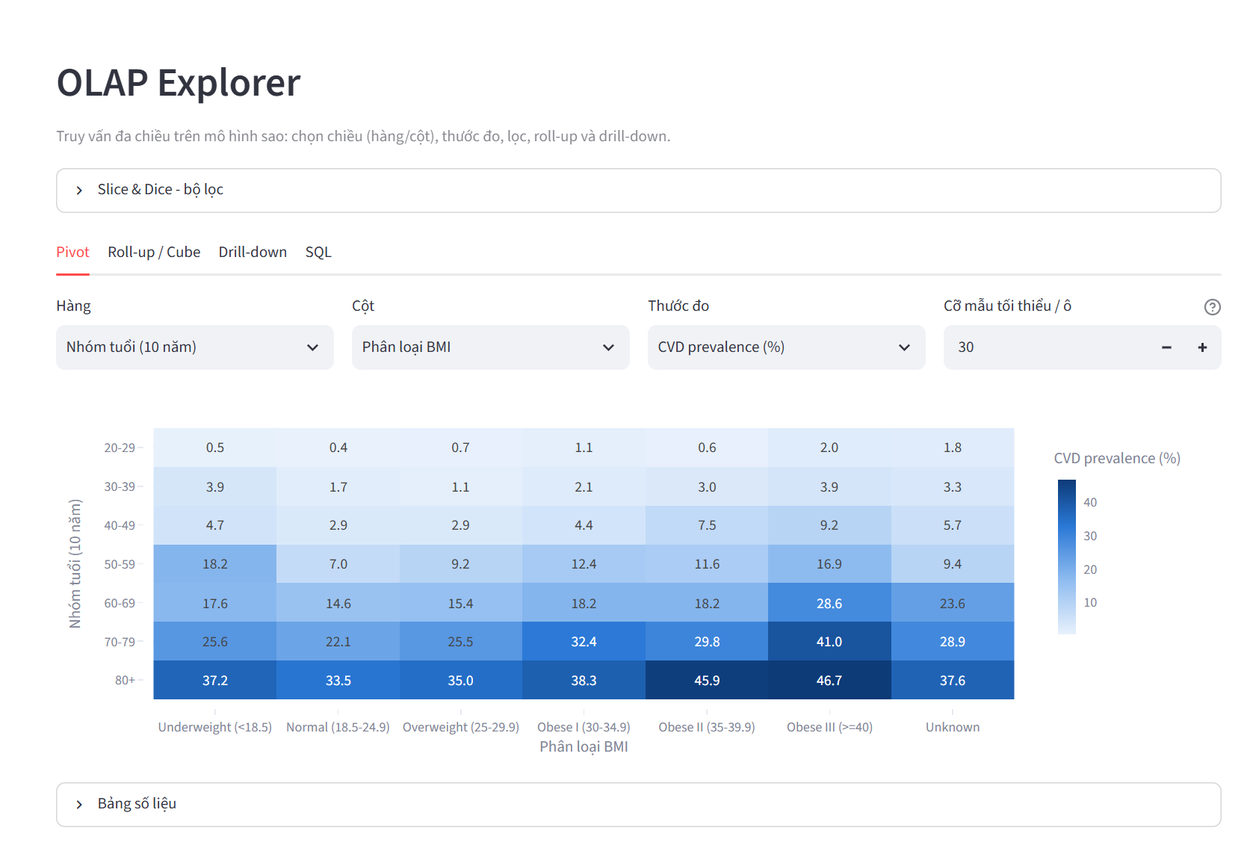
\includegraphics[width=0.7\textwidth]{figures/c_pivot.png}
\caption{OLAP Explorer -- Pivot: tỷ lệ CVD theo nhóm tuổi và phân loại BMI}\label{fig:pivot}
\end{figure}
Trang gồm bốn tab:
\begin{itemize}
\item \textbf{Pivot:} chọn chiều hàng, chiều cột, thước đo và cỡ mẫu tối thiểu mỗi ô; kết quả là bản đồ nhiệt.
\item \textbf{Roll-up / Cube:} bảng kết quả có dòng tổng phụ và tổng chung theo chế độ \emph{rollup}, \emph{cube} hoặc \emph{flat}; có nút tải CSV.
\item \textbf{Drill-down:} khoan từ mức thô xuống mức chi tiết của bảy phân cấp (Thời gian, Tuổi, Chủng tộc, Học vấn, Cân nặng, Huyết áp, Bệnh tim mạch).
\item \textbf{SQL:} ô truy vấn tự do, chỉ chấp nhận một câu \code{SELECT}/\code{WITH}.
\end{itemize}
Khung ``Slice \& Dice'' phía trên lọc theo chín chiều và áp dụng cho cả bốn tab. Các câu truy vấn tương ứng được cung cấp trong file \code{src/sql/truy_van_olap.sql}. Trang này giúp nhà phân tích trả lời nhanh các câu hỏi chưa có sẵn trên dashboard, đồng thời bảo đảm kết quả luôn nhất quán vì dùng chung một lớp truy vấn.

\section{Trang 3: Phân tích yếu tố nguy cơ}
Trang này giúp khám phá các yếu tố đằng sau sự chênh lệch giữa các nhóm (câu hỏi Q3--Q4). Vì tuổi chi phối mạnh nhất tỷ lệ CVD, trang so sánh các nhóm \emph{trong cùng nhóm tuổi} để tránh kết luận sai do khác biệt cấu trúc tuổi.
\begin{figure}[H]
\centering
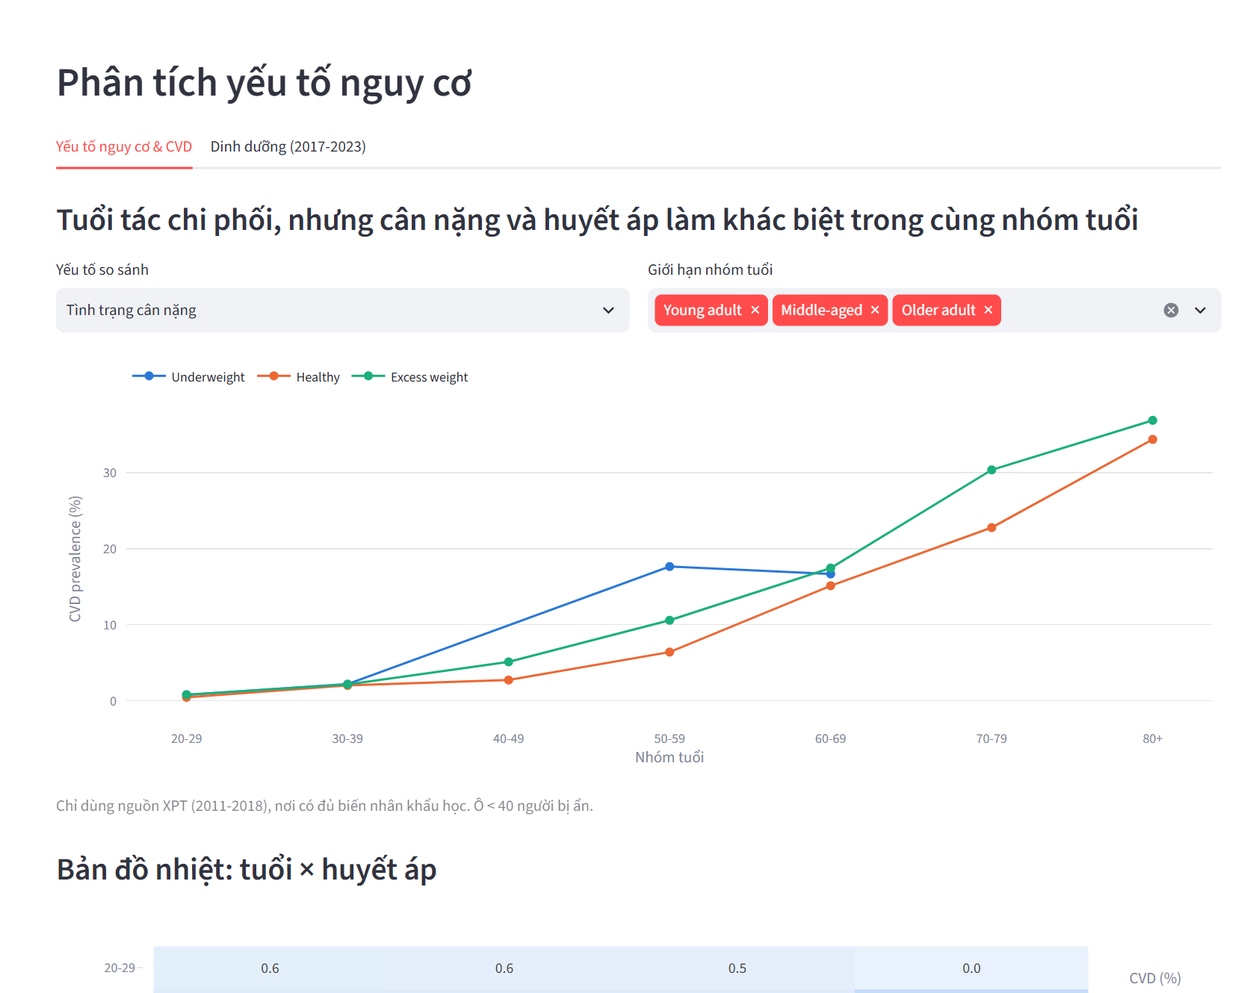
\includegraphics[width=0.7\textwidth]{figures/c_risk.png}
\caption{Trang Phân tích yếu tố nguy cơ}\label{fig:risk}
\end{figure}
Trang gồm hai tab:
\begin{itemize}
\item \textbf{Yếu tố nguy cơ \& CVD:} biểu đồ đường tỷ lệ CVD theo nhóm tuổi, tách theo một yếu tố được chọn (tình trạng cân nặng, nhóm huyết áp, cholesterol, thu nhập hoặc chủng tộc); bản đồ nhiệt nhóm tuổi $\times$ phân loại huyết áp.
\item \textbf{Dinh dưỡng:} so sánh khẩu phần (natri, kali, tỷ lệ Na/K, chất xơ, chất béo bão hòa, đường, cholesterol ăn vào) theo nhóm huyết áp, nhóm CVD, cân nặng, tuổi hoặc chu kỳ.
\end{itemize}
Ví dụ, ở nhóm 60--69 tuổi tỷ lệ CVD là 15,1\% ở người có BMI bình thường và 25,3\% ở người béo phì độ III. Về dinh dưỡng, trung bình mỗi người ăn 3.288 mg natri mỗi ngày; 68,8\% vượt ngưỡng khuyến nghị 2.300 mg và 83,8\% ăn dưới 25 g chất xơ. Trang kèm lưu ý diễn giải: dữ liệu cắt ngang, không có thông tin thuốc nên không suy ra nhân quả.

\section{Trang 4: Hệ hỗ trợ quyết định (DSS)}
Trang DSS dành cho lãnh đạo, chuyên viên chương trình và bác sĩ (câu hỏi Q5--Q8), gồm năm tab (nguyên lý ở Mục~3.7):
\begin{itemize}
\item \textbf{Nguy cơ cá nhân:} nhập tuổi, giới, huyết áp, BMI, cholesterol, HDL; nhận xác suất mắc CVD, mức nguy cơ, so sánh với nhóm cùng tuổi/giới, biểu đồ đóng góp của từng yếu tố và khuyến nghị theo màu (Hình~\ref{fig:individual}).
\item \textbf{What-if:} kéo ba thanh trượt (giảm huyết áp, cholesterol, BMI) và lọc nhóm dân số; xem nguy cơ trước/sau và số ca bệnh tránh được trên 1.000 người (Hình~\ref{fig:whatif}).
\item \textbf{Phân bổ ngân sách:} nhập dân số, chi phí mỗi người, ngân sách và tiêu chí phân khúc; xem xếp hạng phân khúc ưu tiên, độ phủ và so sánh với chia đều (Hình~\ref{fig:budget}).
\item \textbf{Cảnh báo xu hướng:} chọn chiều phân nhóm, chỉ báo và hai chu kỳ; xem biểu đồ thay đổi (cam = tăng, xanh = giảm, xám = ổn định) và bảng thống kê $z$.
\item \textbf{Mô hình:} cỡ mẫu huấn luyện/kiểm tra, AUC, Brier, đường hiệu chuẩn và lý do loại cholesterol, DBP khỏi mô hình.
\end{itemize}
\begin{figure}[H]
\centering
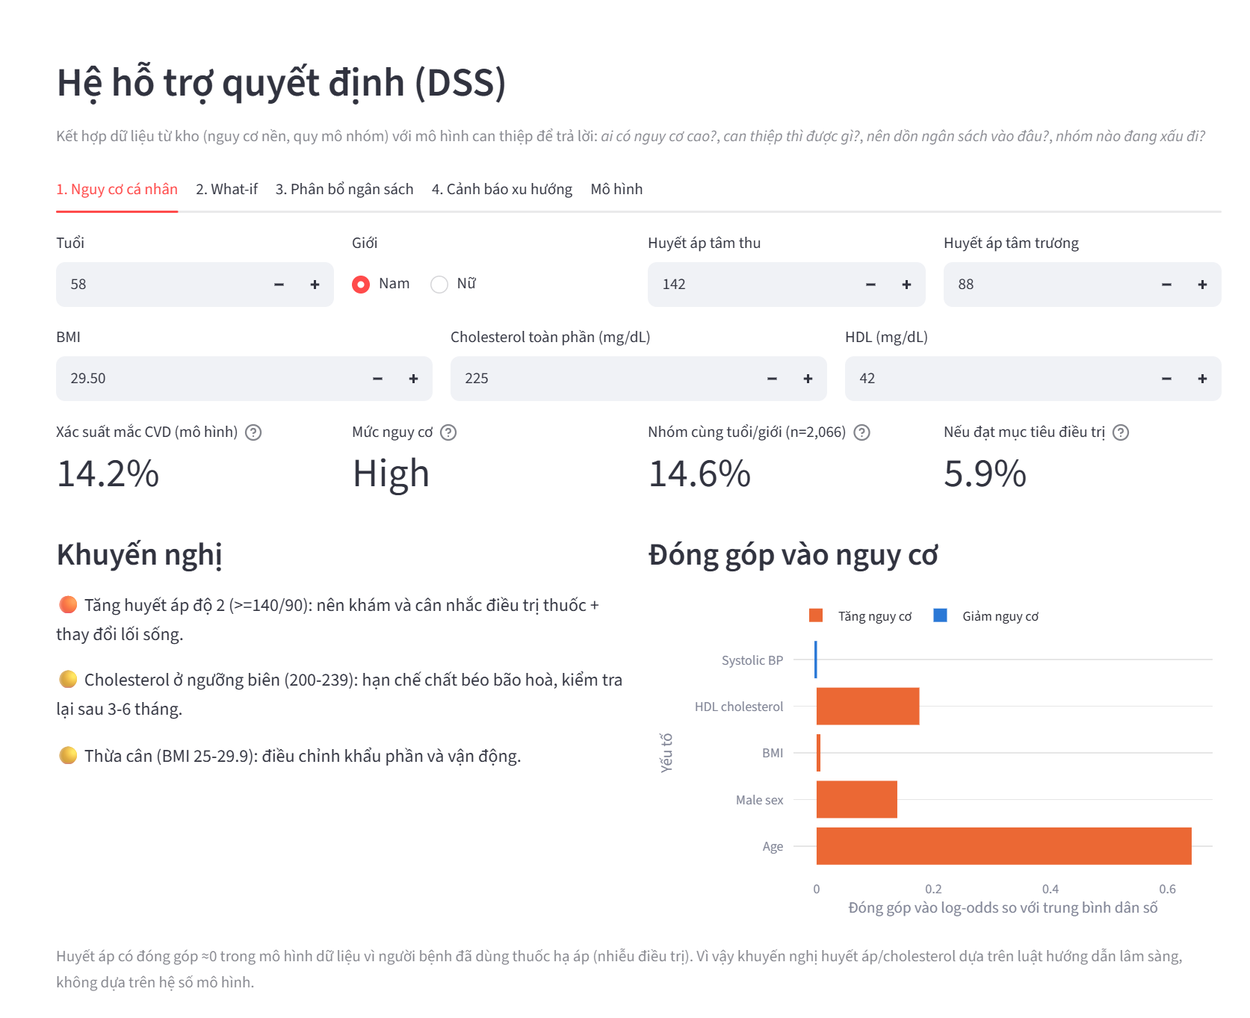
\includegraphics[width=0.62\textwidth]{figures/c_individual.png}
\caption{DSS -- Nguy cơ cá nhân}\label{fig:individual}
\end{figure}
\begin{figure}[H]
\centering
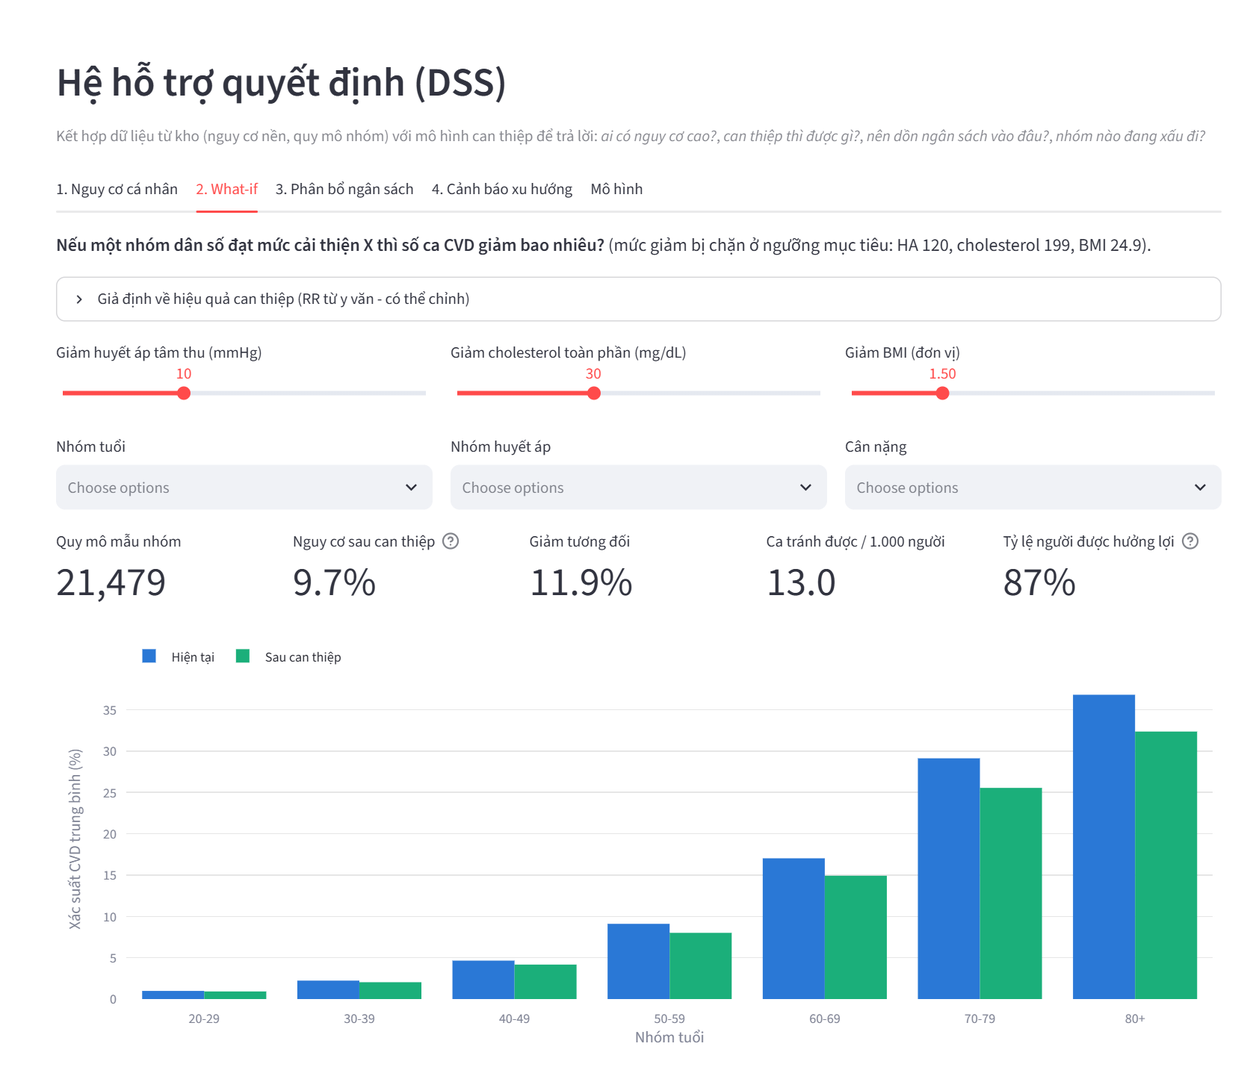
\includegraphics[width=0.62\textwidth]{figures/c_whatif.png}
\caption{DSS -- What-if}\label{fig:whatif}
\end{figure}
\begin{figure}[H]
\centering
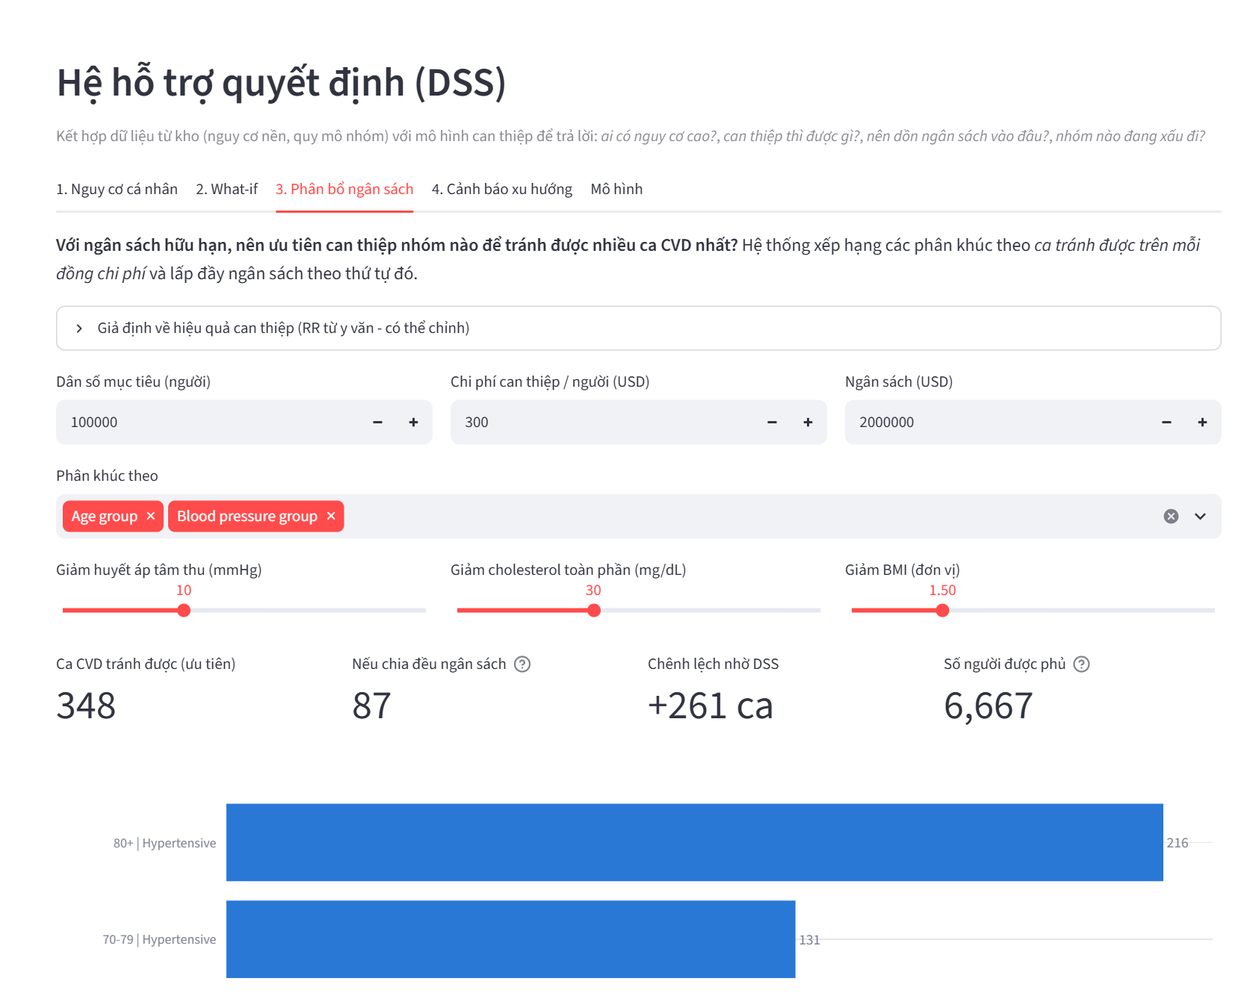
\includegraphics[width=0.62\textwidth]{figures/c_budget.png}
\caption{DSS -- Phân bổ ngân sách}\label{fig:budget}
\end{figure}

\section{Trang 5: Kho dữ liệu \& ETL}
Trang này dành cho nhà phân tích dữ liệu và người cần kiểm tra nguồn gốc số liệu (câu hỏi Q9). Trang gồm bốn tab: \emph{Sơ đồ sao} (sơ đồ và số dòng từng bảng, DDL), \emph{Nhật ký ETL} (số dòng Input, Output và Dropped của từng bước), \emph{Chất lượng dữ liệu} (độ đầy đủ theo chu kỳ, Hình~\ref{fig:dq}) và \emph{Từ điển dữ liệu} (định nghĩa các cờ và measure).
\begin{figure}[H]
\centering
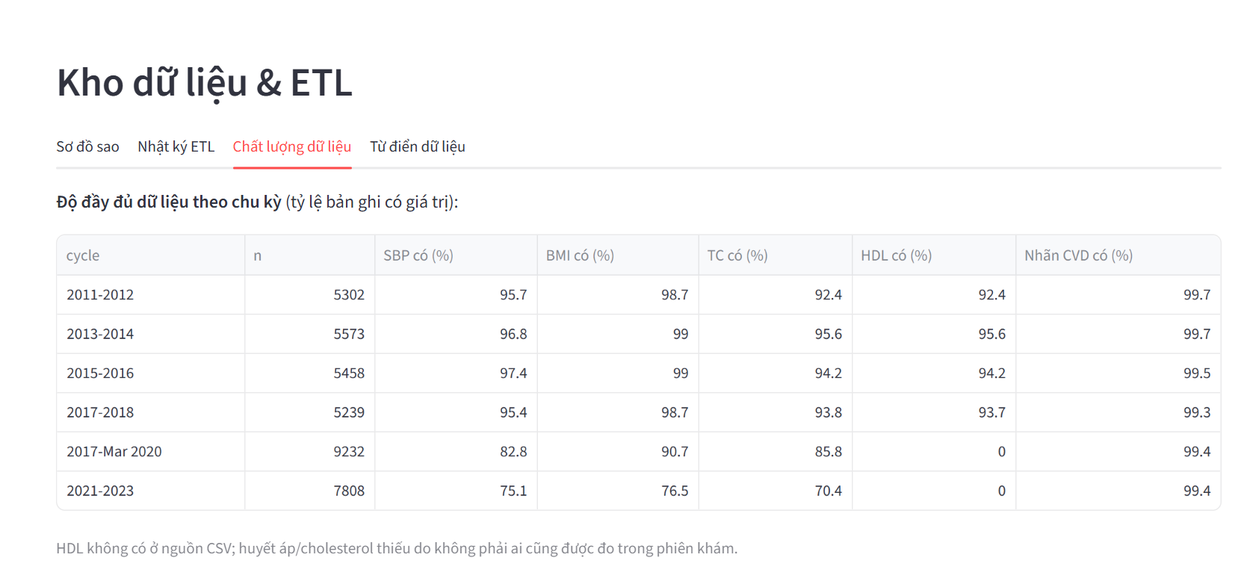
\includegraphics[width=0.7\textwidth]{figures/c_dq.png}
\caption{Trang Kho dữ liệu \& ETL -- độ đầy đủ dữ liệu theo chu kỳ}\label{fig:dq}
\end{figure}

\section{Tính tương tác}
Ứng dụng có các bộ lọc và điều khiển tương tác để phân tích linh hoạt. Các bộ lọc chính gồm:
\begin{itemize}
\item Giới tính và nhóm tuổi (trang Tổng quan)
\item Chu kỳ, giới tính, nhóm tuổi, nhóm chủng tộc, thu nhập, cân nặng, nhóm huyết áp, nhóm CVD, nguồn dữ liệu (khung Slice \& Dice của OLAP Explorer)
\item Yếu tố so sánh và giới hạn nhóm tuổi (trang Phân tích yếu tố nguy cơ)
\item Thanh trượt mức can thiệp, tham số hiệu quả, ngân sách và tiêu chí phân khúc (DSS)
\end{itemize}
Người dùng cũng có thể đặt cỡ mẫu tối thiểu để ẩn các ô quá nhỏ, tải kết quả dạng CSV và truy vấn SQL tự do.

Ứng dụng hỗ trợ một quy trình ra quyết định có cấu trúc:
\begin{enumerate}
\item \textbf{Tổng quan} -- theo dõi tình hình chung và xu hướng.
\item \textbf{OLAP Explorer} -- truy vấn và so sánh các nhóm theo nhiều chiều.
\item \textbf{Phân tích yếu tố nguy cơ} -- tìm yếu tố đằng sau chênh lệch.
\item \textbf{DSS} -- mô phỏng can thiệp, chọn nhóm ưu tiên, đánh giá cá nhân, cảnh báo xu hướng.
\item \textbf{Kho dữ liệu \& ETL} -- kiểm tra nguồn gốc và chất lượng số liệu.
\end{enumerate}
Dòng này giúp người dùng đi từ nhận định mức tổng quan đến phân tích chi tiết và quyết định cụ thể.

\section{Sự phù hợp với bài toán nghiệp vụ}
Ứng dụng giải quyết bài toán nghiệp vụ bằng cách biến các file khảo sát phân mảnh thành một ứng dụng phân tích tương tác. Thay vì phải ghép nối, làm sạch và tính lại số liệu thủ công cho mỗi câu hỏi, người dùng theo dõi chỉ số, so sánh các nhóm, mô phỏng can thiệp và chọn nhóm ưu tiên ngay trên giao diện. Ứng dụng phục vụ các nhóm người dùng khác nhau:
\begin{itemize}
\item \textbf{Lãnh đạo y tế công cộng} dùng trang Tổng quan và trang DSS (phân bổ ngân sách, cảnh báo xu hướng) để giám sát và quyết định ưu tiên.
\item \textbf{Chuyên viên chương trình} dùng what-if và phân bổ ngân sách để so sánh các phương án can thiệp.
\item \textbf{Nhà phân tích dữ liệu} dùng OLAP Explorer, trang Phân tích yếu tố nguy cơ và trang Kho dữ liệu \& ETL để truy vấn tự do và kiểm tra chất lượng.
\item \textbf{Bác sĩ phòng khám} dùng chức năng nguy cơ cá nhân để tư vấn từng người.
\end{itemize}
Việc cung cấp một giao diện tập trung và trực quan giúp tăng khả năng tiếp cận dữ liệu và hỗ trợ ra quyết định dựa trên bằng chứng.

\section{Tóm tắt}
Nhìn chung, ứng dụng đã phát triển cung cấp một công cụ BI và DSS thực tế cho phân tích nguy cơ bệnh tim mạch. Ứng dụng kết nối tới bảng phân tích đã làm sạch trong kho MySQL và trình bày dữ liệu qua năm trang: Tổng quan, OLAP Explorer, Phân tích yếu tố nguy cơ, DSS và Kho dữ liệu \& ETL. Ứng dụng giúp người quản lý theo dõi các chỉ số, so sánh và tìm nguyên nhân chênh lệch giữa các nhóm, mô phỏng can thiệp và chọn nhóm ưu tiên với ngân sách hữu hạn. Mặc dù dữ liệu hiện có giới hạn phạm vi ở tỷ lệ hiện mắc (không có thuốc, chi phí hay biến cố), ứng dụng vẫn chứng minh cách BI và các công nghệ liên quan biến dữ liệu khảo sát có cấu trúc thành thông tin hỗ trợ quyết định hữu ích.
